% !TeX program = latexmk
% !TeX spellcheck = pl_PL
% !TeX root = example.tex

\chapter{Najczęściej wykorzystywane narzędzia w zarządzaniu projektami}

Zarządzanie projektami informatycznymi ściśle wiąże się z wykorzystaniem narzędzi informatycznych,
które wspomagają ten proces. Przy ich wyborze warto pamiętać, iż mają pomagać w pracy projektowej,
a nie przeszkadzać w jej realizacji, dlatego należy wybierać je mądrze.
Przykładem nieodpowiedniego doboru narzędzia może być sytuacja,
w której kierownik projektu nie dotrzymuje terminów swoich prac,
ze względu na zajmowanie się raportowaniem postępu prac lub aktualizacją harmonogramu.
\cite{Kopczewski_2015}

\section{Narzędzia wspomagające podejście klasyczne}

\subsection{Microsoft Project}

Najbardziej popularnym narzędziem stosowanym w metodykach klasycznych jest Microsoft Project (\ref{rys:project}).
Pozwala on na rozpisanie całego harmonogramu działań, zaplanowanie budżetu czy stworzenie wykresu Gantta,
tak niezbędnego w pracy kierownika. Pozwala także na tworzenie raportów, prezentacji i wykresów z postępów prac.

\begin{figure}[H]
	\centering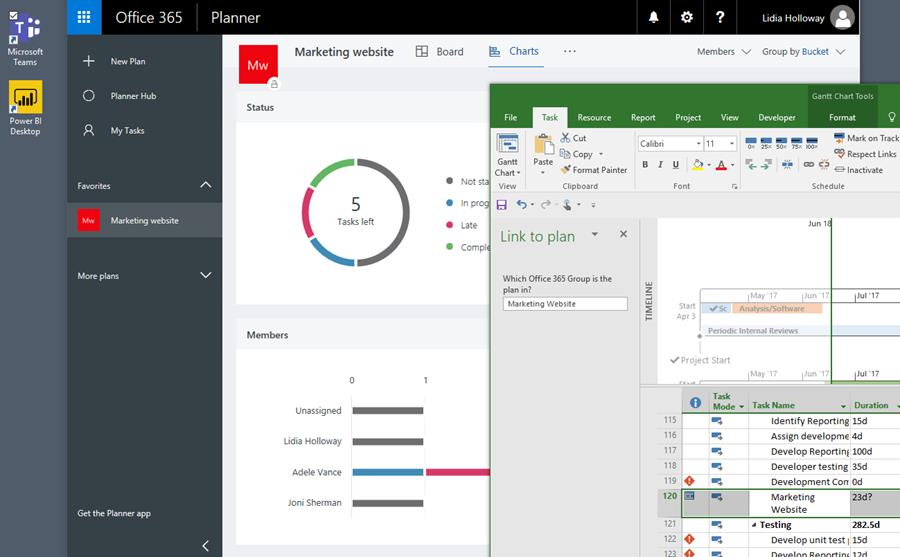
\includegraphics[width=.8\textwidth]{img/Microsoft_Project}
	\caption{Microsoft Project[www.microsoft.com]}\label{rys:project}% Źródło rysunku i etykieta przez którą odwołujemy się do rysunku.
\end{figure}

\subsection{Gantt Project}

W niektórych przedsiębiorstwach w zarządzaniu projektami używa się programu GanttProject.
Jest to darmowe narzędzie umożliwiające dynamiczne tworzenie diagramów Gantta
z podziałem na poszczególne zadania wraz z rozplanowaniem ich w czasie.
Dodatkowo pozwala ono na tworzenie wykresów PERT (ang. Program Evaluation and Review Technique)
wraz ze ścieżkami krytycznymi.
\cite{Trendy_Zarzadzanie}


\section{Narzędzia stosowane w metodykach zwinnych}

W małych zespołach projektowych, które wykorzystują metodyki zwinne,
odchodzi się zazwyczaj od Microsoft Project czy GanttProject stosując aplikacje webowe.
Przykładem takich aplikacji są: Jira, Mantis, TFS, Trello, Redmine, Kanban Tool.

Przy metodykach zwinnych, właściciel produktu tworzy rejestr produktowy (ang. Product Backlog),
który ma formę listy zawierającej wymagania klienta z określoną wagą (priorytetem) i czasochłonnością.
\cite{Shwaber_2004}

Wymienione wyżej narzędzia pozwalają na taką pracę i umieszczanie danych w chmurze,
dzięki czemu każdy członek zespołu ma do nich dostęp,
niezależnie od lokalizacji, czy pracuje w biurze czy poza nim.
Zadania w backlogu
\footnote{Backlog – rejestr sprintu / lista zadań \cite{metody_zwinne_2016}}
powinny być rozpisane dla obecnego sprintu
\footnote{Sprint – jeden z etapów niektórych metodyk zwinnych, który wyznacza rytm pracy. W jego
trakcie następuje faktyczne wykonanie określonej funkcjonalności \cite{Samoorganizacja_2010}}
oraz zawierać dodatkowe zadania, które będą zasilać kolejny sprint bądź zostaną wykonane w istniejącym,
gdy nadarzy się taka możliwość.

Takie podejście do pracy umożliwia wykonanie części zadań przed wyznaczonym czasem.
Narzędzia te pozwalają również na przypisanie konkretnego zadania do danego użytkownika,
dzięki czemu każdy pracownik zna zakres swojej odpowiedzialności.
Zapobiega to przypadkowemu wykonaniu tego samego zadania przez kilka osób.

Niektóre firmy, a można nawet powiedzieć, że wiele firm,
niezależnie od wykorzystywanej metodyki używa narzędzie Microsoft Excel do zarządzania projektami.
Umożliwia ono przedstawienie danych w postaci tabeli oraz różnych grafów.
Każda firma może zarządzać nim na swój własny sposób, dzięki czemu proces ten jest bardzo elastyczny.
Ponadto ułatwia on wykonanie prognoz przyszłych dochodów, kalkulacji wybranych parametrów i wskaźników.

Kolejnym narzędziem wykorzystywanym na szeroką skalę jest SharePoint,
który umożliwia współdzielenie plików czy tworzenie listy zadań,
która może być wykorzystana w MS Project.

\section{Narzędzia wspomagające proces estymacji zadań projektowych}

W klasycznych projektach tworzymy harmonogramy, szczegółowe plany, gdzie mamy daty,
gdzie mamy godziny, gdzie każde zadanie ma określony czas realizacji.
W przypadku projektów zwinnych często odchodzimy od tak szczegółowego planowania.
ale jakaś forma planowania oczywiście jest potrzebna.
W projektach zwinnych bardzo często planujemy bez użycia dni i godzin.
Dlatego stosujemy różne alternatywne metody i jedną z takich alternatywnych metod
jest metoda zwana Team Estimation Game.

\subsection{Team Estimation Game}

Team Estimation Game działa tak:

\begin{itemize}
	\item Członkowie zespołu kolejno pobierają kartę ze stosu i przyklejają ją do ściany.
	Każda karta przedstawia jedną historyjkę.
	Po umieszczeniu pierwszej karty w środku, każdy członek zespołu umieszcza swoją kartę po prawej,
	jeśli jest trudniejsza, po lewej, jeśli jest mniej trudna,
	lub pod inną kartą, jeśli historyjki są mniej więcej takiej samej złożoności
	(patrz \ref{rys:teamEstimationGame}).
	\item Użytkownik może użyć swojej kolejki, aby przesunąć kartę już na ścianie po prawej lub lewej stronie.
	\item Proces może być kontynuowany po tym, jak stos kart zostanie zużyty,
	aż do ogólnego konsensusu w rankingu kart. Gracze mogą omawiać historie i wpływać na swoje decyzje.
	\item Następnie każdy członek drużyny odbiera kartę z numerem i umieszcza ją na jednej z kolumn.
	Członek zespołu może użyć swojej kolejki, aby zmienić przypisanie numeru
	wykonane przez innego członka zespołu. Trwa to aż do osiągnięcia konsensusu.
\end{itemize}

\begin{figure}[H]
	\centering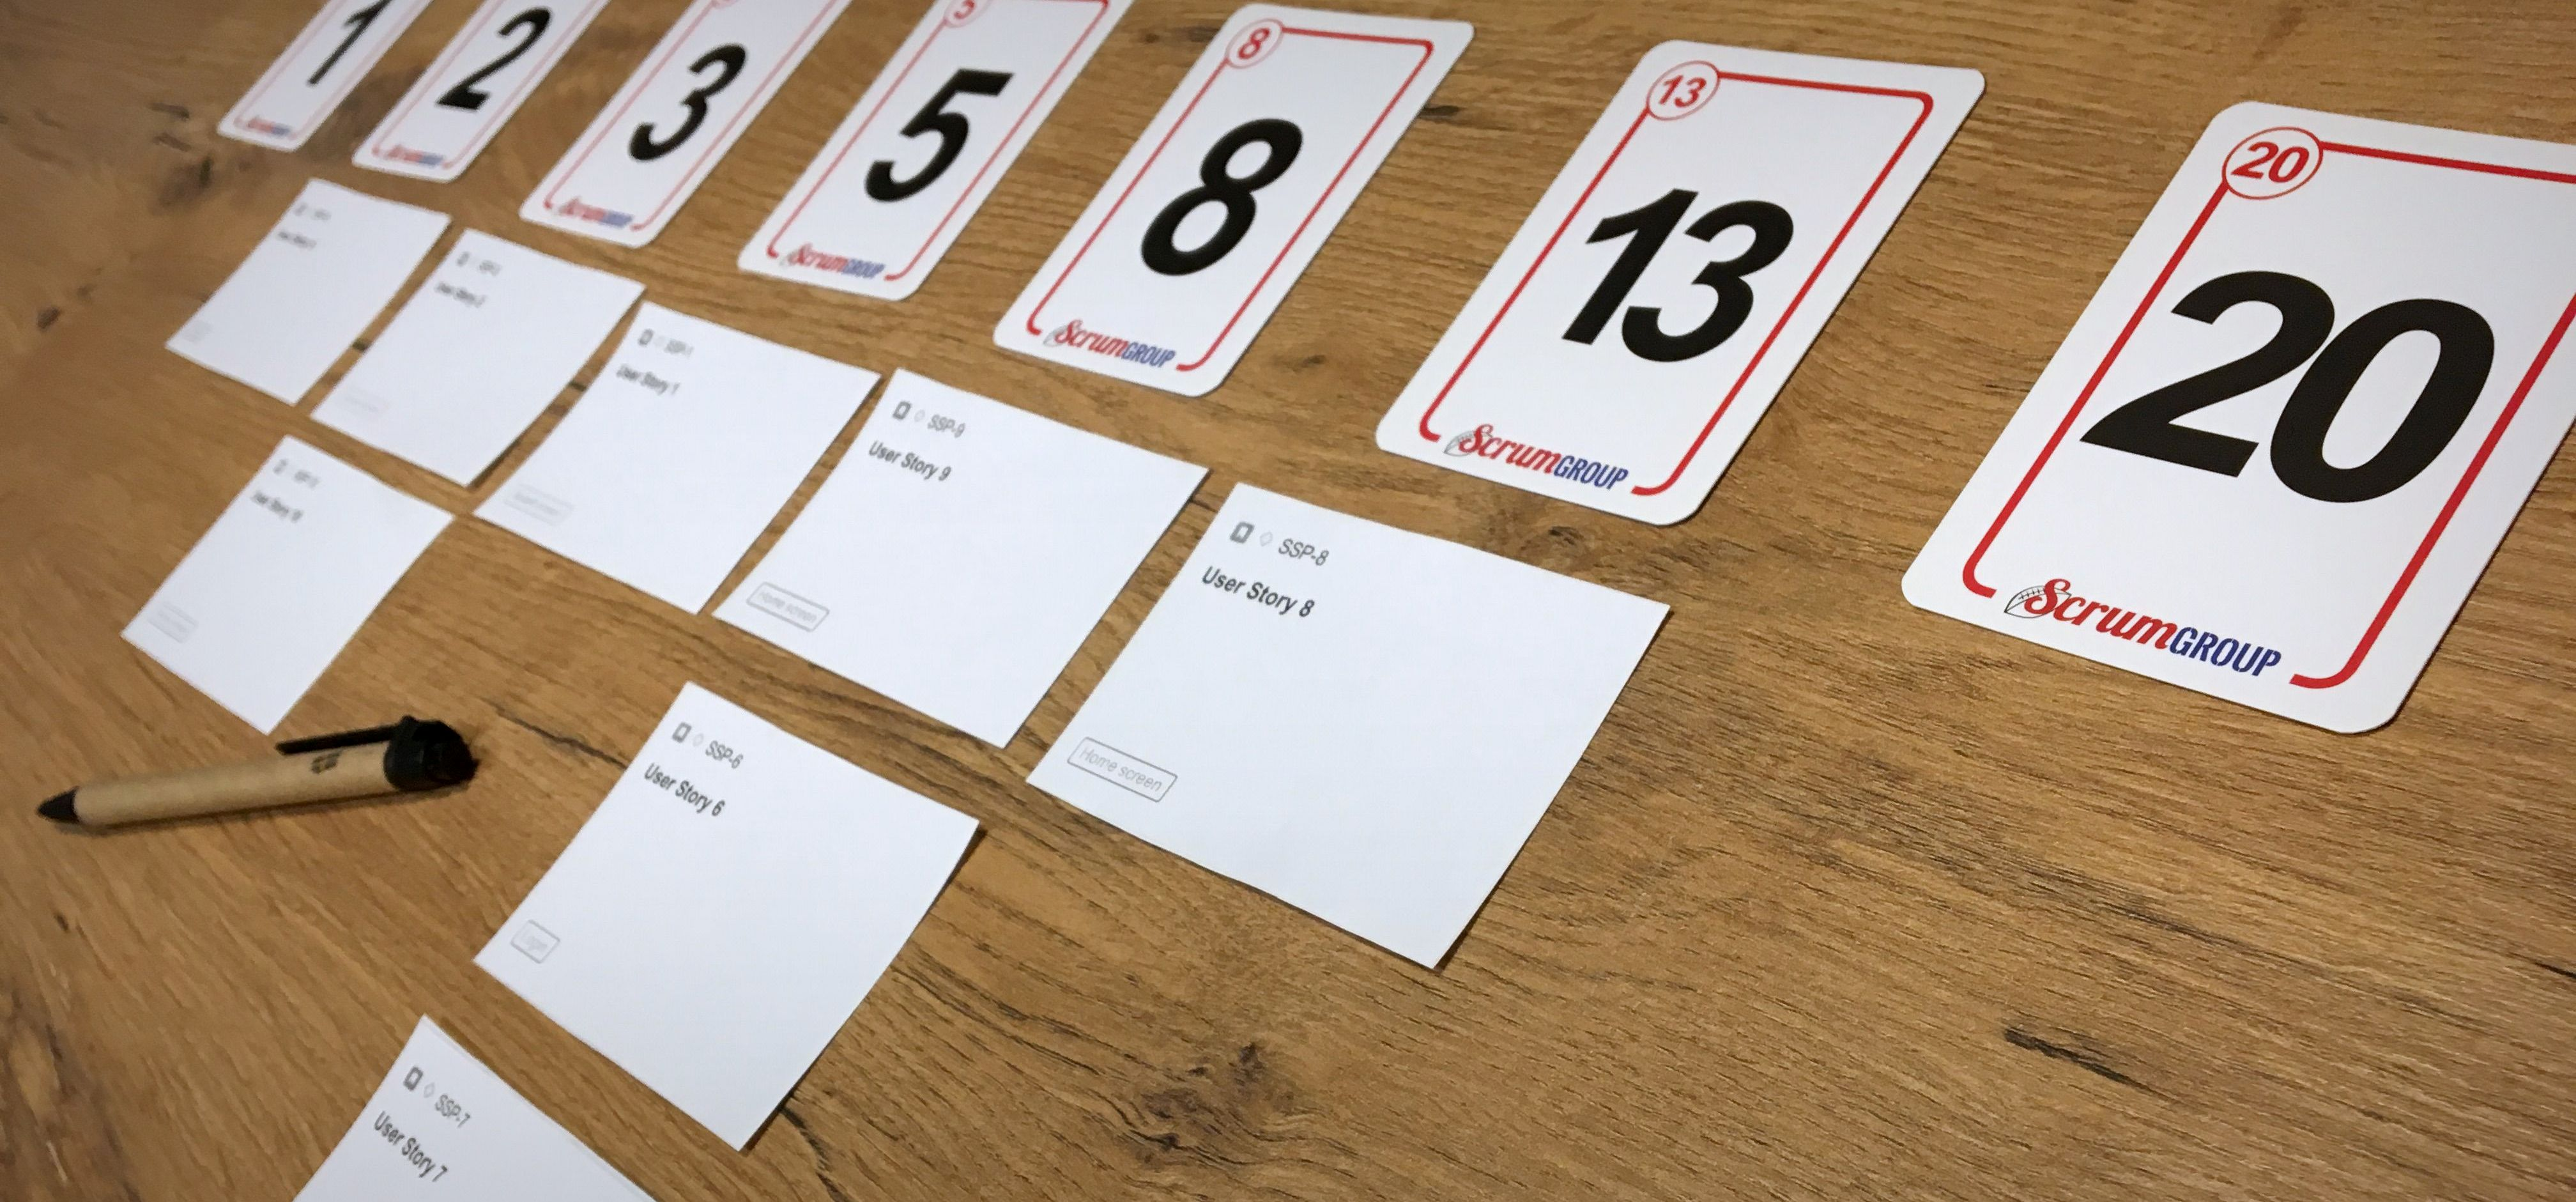
\includegraphics[width=.6\textwidth]{img/team_estimation_game}
	\caption{Team Estimation Game [www.scrum-master.pl]}
	\label{rys:teamEstimationGame}
\end{figure}

Zbiór liczb zawiera tylko te w sekwencji Fibonacciego, aby odzwierciedlić ogólną zasadę,
że ryzyko wzrasta geometrycznie proporcjonalnie do złożoności.

\subsection{Kanban}

Inną z takich alternatywnych metod jest metoda Kanban. Kanban, to koncepcja wzięta z produkcji,
która została świetnie zaadaptowana właśnie do zarządzania projektami zwinnymi.
Kanban w przypadku projektów jest po prostu tablicą, na której pokazujemy,
rejestrujemy to, co się dzieje w projekcie (patrz \ref{tabela:kanban}).

Zaczynając od lewej strony tej tablicy, mamy backlog produktu, a więc wszystkie nasze historyjki,
które określają to, co jest w projekcie do realizacji.
Następnie mamy trzy główne etapy realizacji projektu, w których nasze historyjki będą się za chwilę znajdowały:

\begin{itemize}
	\item Pierwszym takim etapem jest \textit{breakdown} albo \textit{analysis}, czyli analizowanie historyjek,
	rozbijanie ich na mniejsze części, na zadania, analiza tego co jest do zrobienia, w jaki sposób mamy te zadania zrealizować.
	W tym miejscu musimy także zastanowić się nad kompatybilnością i powiązaniami pomiędzy poszczególnymi zadaniami,
	a także nad priorytetami. Dlatego bierzemy przede wszystkim te rzeczy, które mają wysoki priorytet oraz wszystkie funkcje,
	które są z nimi powiązane, abyśmy mogli dostarczyć nowy produkt.
	\item Kolejny etap, to jest rozwój (ang. \textit{develop}) - w sytuacjach, gdzie opracowujemy nasz projekt,
	a więc tutaj zespół tworzy faktycznie te rozwiązania, które miały być opracowane.
	\item Trzeci etap, to \textit{validate}, czyli kontrola, testy, ocena tego, co zostało zrobione.
	Sprawdzamy czy rzeczywiście to, co miało być osiągnięte, zostało osiągnięte.
	Jeżeli tak, możemy dołączyć te funkcjonalności do produktu i przekazać je do klienta.
\end{itemize}

W każdym z tych etapów widzimy co najmniej dwie kolumny:

\begin{itemize}
	\item jedna kolumna, to \textit{working}, czyli pracujemy nad czymś,
	\item druga kolumna, to \textit{done}, czyli "wykonane" - wykonaliśmy to zadanie
	i dalej zadanie może przejść do kolejnego etapu, do kolejnej części prac.
	\item Dodatkowo, w przypadku kolumny związanej z rozwojem, mamy taką kolumnę \textit{track}
	– to sytuacja, w której opracowaliśmy jakąś funkcjonalność,
	ale nie jesteśmy jej w stanie wdrożyć dalej, ponieważ czekamy na opracowanie innych,
	powiązanych z nią funkcjonalności.
	Czasem jest tak, że pewna funkcjonalność może być już gotowa, ale nie może działać,
	dopóki inne elementy nie zostaną przygotowane.
	Dlatego jest takie pole oczekiwania na inne elementy, które muszą być przygotowane.
\end{itemize}

\begin{table}
	\centering\caption{Tablica w metodzie Kanban.}\label{tabela:kanban}
	\begin{tabular}{*8{l} }% wyrównanie kolumn tabeli -> l c r - do lewej, środka, do prawej
	\toprule
	\multicolumn{1}{|c|}{\textbf{Backlog}} &\multicolumn{2}{|c|}{\textbf{Breakdown (10*)}} & \multicolumn{3}{|c|}{\textbf{Develop (15*)}} & \multicolumn{2}{|c|}{\textbf{Validate (10*)}} \\
	\midrule
	Epics,User Stories & Working
	& Done & Working & Track & Done & Working & Done \\
	\bottomrule
	\end{tabular}
\end{table}

Widzimy więc, że w tej metodyce nie mamy iteracji jako takich, mamy stały przepływ historyjek,
stały przepływ pracy, która jest realizowana w naszym projekcie.
Ale ktoś może zapytać, w jaki sposób razie określamy poziom wykonania prac, w jaki sposób określamy
ile tej pracy możemy mieć jednocześnie rozpoczętej?
Temu służą te liczby w nawiasach, które widzimy w nagłówku tabeli.
Te liczby określają nam liczbę punktów, które mogą być aktualnie w obróbce.

Historyjki oceniamy nie względem czasu, lecz względem punktów trudności,
punktów zaangażowania, które jest niezbędne, aby daną funkcję zrealizować.
Jeżeli zatem w danym etapie naszej tablicy Kanban mamy dopuszczone 10 punktów,
to znaczy, że możemy tam mieć w trakcie obróbki historyjki,
których suma punktów estymacji nie przekracza 10-ciu. Tak samo w kolejnych etapach.
Zatem to określa nam poziom pracy, która jest wykonywana i powoduje, że praca będzie przebiegać płynnie,
nie będzie korków, nie będzie zatrzymań i będziemy w stanie w odpowiednim czasie dostarczać klientowi
nowe produkty.

\subsection{Planning Poker}

Jeszcze inną z takich alternatywnych metod (bardzo popularną) jest metoda,
której poświęcona jest niniejsza praca.
Ta metoda nazywa się \textit{Planning Poker} i pozwala nam oszacować trudność,
czasochłonność poszczególnych zadań, które są do wykonania w ramach projektu.
Ta metoda ma też tą zaletę, że integruje zespół i pozwala uwzględnić różne punkty widzenia,
a także przyczynia się do lepszego zrozumienia zadań, które są do wykonania.
O co w tej grze chodzi? Bazujemy tutaj z grubsza na liczbach z ciągu Fibonacciego (patrz \ref{rysunek:poker}).

Określamy trudność poszczególnych zadań wykorzystując kolejne liczby z tego ciągu: 1, 2, 3, 5, 8,13, 21 itd.
Jeżeli jakieś zadanie oceniliśmy na 5, to znaczy, że jest ono trudniejsze od zadania, które oceniliśmy na 3,
ale ile ono zajmie? Tego nie wiemy, to nas chwilowo nie interesuje.
Staramy się określić, przede wszystkim, na ile trudne i na ile pracochłonne, naszym zdaniem, mogą być zadania.

Praktyka pokazuje, że planując sprinty, wcale nie musimy mieć szczegółowych informacji na temat czasu,
te informacje zresztą często się nie sprawdzają.
Taka forma punktowa zupełnie nam wystarcza. Kiedy wiemy, ile jesteśmy w stanie w ciągu sprintu
zrealizować takich punktów, to wówczas jesteśmy w stanie stwierdzić, ile możemy zadań w danym sprincie upchnąć.

Rozgrywka Planning Poker odbywa się następująco:

\begin{itemize}
	\item Zespół programistów spotyka się na spotkaniu, siada przy stole,
	każdy otrzymuje swoje karty i mamy pakiet zadań (czy pakiet historyjek) z backlogu,
	którymi się musimy zająć.
	Zazwyczaj spotkanie prowadzi scrum master lub właściciel produktu (ang. Product Owner),
	przedstawia on historyjkę, którą mamy się zająć, określa czego ona dotyczy.
	\item Następnie każdy z członków zespołu wyciąga kartę, która jego zdaniem dobrze określa trudność,
	realizacji tego zadania i kładzie ją na stole tak, aby nie było widać tej liczby.
	\item Kiedy wszyscy są gotowi, odwracamy karty i patrzymy czy wynik, który uzyskaliśmy jest zgodny,
	czy też nie. Jeżeli wszyscy pokazali praktycznie tą samą liczbę, to sprawa jest załatwiona.
	To znaczy, że wszyscy rozumiemy zadanie w taki sam sposób, tak samo oceniamy jego trudność
	i możemy przejść do kolejnego.
	\item Kiedy jednak występuje zróżnicowanie, konieczna jest dyskusja.
	Pytamy osoby, która podała najniższą liczbę, dlaczego tak uważa.
	Pytamy osoby, która podała najwyższą liczbę, dlaczego tak uważa.
	Bardzo często te różnice wynikają z tego, że nie do końca rozumiemy zadanie.
	Po dyskusji, gdy żaden z członków zespołu nie ma już wątpliwości co do
	szczegółów omawianego zadania, można powtórzyć rozgrywkę, która zazwyczaj dzięki
	odbytej dyskusji, kończy się konsensusem.
\end{itemize}

\begin{figure}[H]
	\centering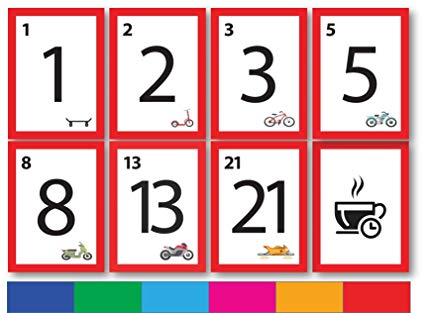
\includegraphics[width=.6\textwidth]{img/Planning_Poker}
	\caption{Przykładowe karty do Planning Pokera}\label{rysunek:poker}
\end{figure}

A więc Planning Poker pozwala nam lepiej zrozumieć zadania w zespole,
dzięki czemu nie ma później nieporozumień i dzięki czemu to planowanie jest bardziej precyzyjne.
Kiedy przejdziemy przez wszystkie historyjki i odzwierciedlimy, oszacujemy ich trudność w punktach,
możemy przejść do planowania sprintu.

Z doświadczenia wiemy, że nasz zespół jest w stanie zrealizować określoną liczbę punktów w ciągu danego sprintu.
Ta liczba nazywa się \textit{team velocity}, czyli szybkość, z jaką zespół pracuje.
Jest typowa dla każdego zespołu, a więc nie jest tak, że jeżeli jeden zespół
jest w stanie zrealizować 30 punktów, to każdy inny będzie w stanie tyle samo zrealizować.

Co więcej, nie można tej liczby traktować jako wskaźnika motywacji
(zróbcie pięć punktów więcej, to dostaniecie premię) dlatego,
że zaobserwowano, iż w takich przypadkach każde kolejne szacowanie po prostu powoduje,
że członkowie zespołu przydzielają więcej punktów, czyli określają zadania jako trudniejsze,
niż są w rzeczywistości, a więc mamy taką inflację punktów - nie ma realnego
zwiększenia realnego wykonanej pracy, jest po prostu zwiększenie liczby punktów.
Taki sposób motywacji nie jest zatem dobrym pomysłem.

Dzięki tej metodzie możemy odejść od określania, czy coś będzie trwało 2,5 godziny,
czy 3,5 godziny, możemy skupić się na lepszym zrozumieniu zadań,
jak również na tym, aby lepiej rozplanować pracę.
